\documentclass[t, 11pt]{beamer}
\pdfmapfile{+sansmathaccent.map}
%%% Работа с русским языком
\usepackage{cmap}				
\usepackage{mathtext} 				
\usepackage[T2A]{fontenc}		
\usepackage[utf8]{inputenc}			
\usepackage[english,russian]{babel}	

\usetheme{Ilmenau}
\usecolortheme{lily} % Цветовая схема



%%% Работа с картинками
\usepackage{graphicx}

\usepackage{csquotes}

\hypersetup{				
	colorlinks=true,       	
	linkcolor=blue,          
	citecolor=blue,       
	filecolor=magenta,      
	urlcolor=magenta           
}


\title{Языковые модели}
\subtitle{Language models}
%\author{Чувакин Сергей}
\date{15.10}
%\institute[<<Анализ больших данных в бизнесе, экономике и обществе>>]{<<Высшая школа экономики>>}
\institute{<<Высшая школа экономики>>}
\begin{document}
	\frame[plain]{\titlepage}
	\section{Outline}
	
	\begin{frame}
		\frametitle{\insertsection} 
		\begin{block} {}
			 
			\hyperlink{l1}{\beamerbutton{Language models}}
		\end{block}
			\begin{block}{}
		\hyperlink{l2}{\beamerbutton{Probabalistic}}
		\end{block}
				\begin{block}{}
		\hyperlink{l2}{\beamerbutton{Perplexity}}
		\end{block}
	\end{frame}
	

\subsection{Language models} 
\begin{frame} \label{l1}
	\frametitle{\insertsection}
	\frametitle{\insertsubsection}  
	Language model (LM) - model that predict a next word given a previous. 
\end{frame}


\begin{frame}
	\frametitle{\insertsection}
	\frametitle{\insertsubsection}  
	\begin{itemize}
		\item \textbf{Machine translation}: translating a sentence saying about height it would probably state that $P(tall man)>P(large man)$ as the ‘large’ might also refer to weight or general appearance thus, not as probable as ‘tall’
		\item \textbf{Spelling Correction}: Spell correcting sentence: “Put you name into form”, so that $P(name into form)>P(name into from)$
		\item \textbf{Speech Recognition}: Call my nurse: $P(Call my nurse.)\gg P(coal miners)$, I have no idea. $P(no idea.)\gg P(No eye deer.)$
		\item Summarization, question answering, sentiment analysis etc.
	\end{itemize}
\end{frame}


\begin{frame}
	\frametitle{\insertsection}
	\frametitle{\insertsubsection}  
	\begin{itemize}
		\item Statistical Language Models
		\item Neural Language Models
	\end{itemize}
\end{frame}
\subsection{Probabilistic language modeling}




	\begin{frame} \label{l2}
	\frametitle{\insertsection}
	\frametitle{\insertsubsection}
	
	Sentence:
	
	\vspace{1cm}
	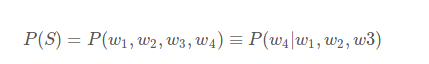
\includegraphics[width=0.7\linewidth]{sent.png}
	
	\vspace{1cm}
	
	
\includegraphics[width=1\linewidth]{chain_rule.png}
	
		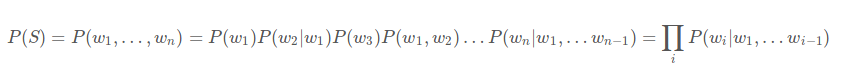
\includegraphics[width=1\linewidth]{sent_chain.png}
\end{frame}


	\begin{frame}
	\frametitle{\insertsection}
	\frametitle{\insertsubsection}
	
	Initial way
	
	\vspace{1cm}
	
\includegraphics[width=0.9\linewidth]{1.png}
	
	\vspace{1cm}
	
	Markov assumption:
	
\includegraphics[width=1\linewidth]{mark_a.png}
	
\end{frame}

\begin{frame}
	\frametitle{\insertsection}
	\frametitle{\insertsubsection}
	
	Bi-gram model
	
	\vspace{1cm}
	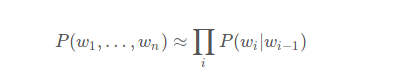
\includegraphics[width=0.6\linewidth]{2.png}
	
	\vspace{1cm}
	
	Maximum Likelihood Estimate (MLE)
	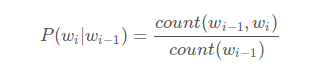
\includegraphics[width=0.6\linewidth]{mle.png}
	
\end{frame}

\subsection{Information measure}

\begin{frame} \label{l3}
	\frametitle{\insertsection}
	\frametitle{\insertsubsection}
To remind:	
\begin{itemize}
	\item Surprisal
	\item Entropy
	\item Cross-Entropy
	\item Cross-Entropy Loss
	\item Perplexity
\end{itemize}
\end{frame}

\begin{frame}
	\frametitle{\insertsection}
	\frametitle{\insertsubsection}
	Surprisal
	%Now, if yi is the probability of ith outcome then we could represent surprisal (s) as:
	
\includegraphics[width=1\linewidth]{surp.png}	
	
	\vspace{0.5cm}
	Entropy
%Now, if yi is the probability of ith outcome then we could represent surprisal (s) as:

\includegraphics[width=1\linewidth]{entropy.png}
\end{frame}


\begin{frame}
	\frametitle{\insertsection}
	\frametitle{\insertsubsection}
	Cross-Entropy
	%Now, if yi is the probability of ith outcome then we could represent surprisal (s) as:
	
\includegraphics[width=1\linewidth]{cross_en.png}	
	
	\vspace{0.3cm}
	Cross-Entropy Loss
	%Now, if yi is the probability of ith outcome then we could represent surprisal (s) as:
	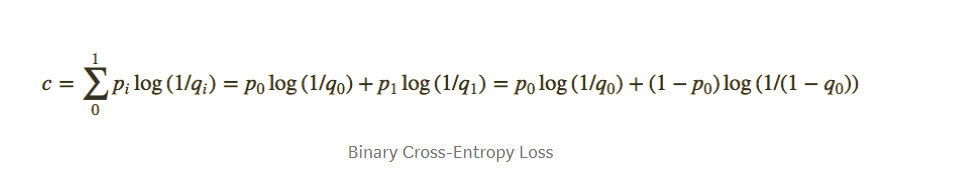
\includegraphics[width=1\linewidth]{bi_loss.png}
\end{frame}

\begin{frame}
	\frametitle{\insertsection}
	\frametitle{\insertsubsection}
	Perplexity
	%Now, if yi is the probability of ith outcome then we could represent surprisal (s) as:
	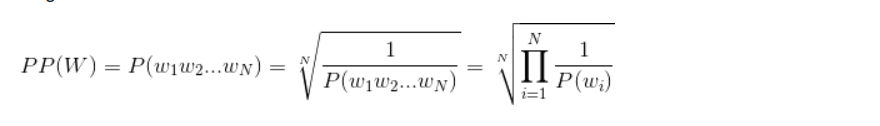
\includegraphics[width=1\linewidth]{perpl.png}	
	
\end{frame}




%	\begin{frame}
%	\frametitle{\insertsection}
%	\frametitle{\insertsubsection}  
%	Синонимы кватификаторов 
%	\begin{center}
%		\begin{table}[]
%			\begin{tabular}{c|c|c}
%				\hline 	
%				\hline
%		+ & 1 и более раз &\{1,\}   \\
%		* & 0 и более раз &\{0,\}   \\
%
%		? &  0 или 1 раз& \{0,1\}  \\
%  
%			\end{tabular}
%		\end{table}
%	\end{center}
%\end{frame}

%\begin{frame}
%	\frametitle{\insertsection}
%	\frametitle{\insertsubsection}  
%	Чтобы убрать жаность необходимо добавить ?
%	
%	\vspace{0.5cm}
%	
%	Строка на вход  <<( dfghvb ) sdvsd ( sdcvkjnh ) sdvsd ( dkjhvgr ) sdvfv.>>
%	
%	\vspace{0.5cm}
%	
%	шаблон: r"$\backslash$(.+?$\backslash$)"
%	
%	\vspace{0.5cm}
%	
%	на выходе: ['dfghvb', 'sdcvkjnh', 'dkjhvgr']
%	
%\end{frame}



%	\begin{frame}
%	\frametitle{\insertsection}
%	\frametitle{\insertsubsection}
%	
%	
%	\vspace{1cm}
%	\includegraphics[width=0.9\linewidth]{page2.png}
%	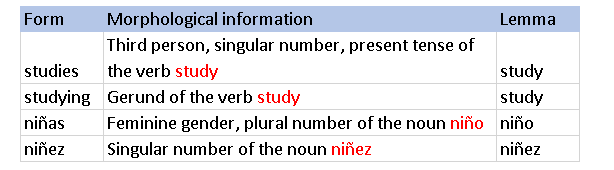
\includegraphics[width=0.7\linewidth]{lem.png}
%\end{frame}
\end{document}